\documentclass{article}
\usepackage[utf8]{inputenc}
\usepackage[a4paper, total={6.5in, 9.5in}]{geometry}


\usepackage[spanish]{babel}

\usepackage{graphicx}
\usepackage{placeins}

\usepackage{hyperref}
\usepackage{subcaption}


\usepackage{amsfonts}
\usepackage{amsmath}

\usepackage{minted}

\begin{document}

%%%%%%%%%%%%%%%%%%%%%%%%%%%%%%%%%%%%%%%%%
% University Assignment Title Page 
% LaTeX Template
% Version 1.0 (27/12/12)
%
% This template has been downloaded from:
% http://www.LaTeXTemplates.com
%
% Original author:
% WikiBooks (http://en.wikibooks.org/wiki/LaTeX/Title_Creation)
%
% License:
% CC BY-NC-SA 3.0 (http://creativecommons.org/licenses/by-nc-sa/3.0/)
% 
% Instructions for using this template:
% This title page is capable of being compiled as is. This is not useful for 
% including it in another document. To do this, you have two options: 
%
% 1) Copy/paste everything between \begin{document} and \end{document} 
% starting at \begin{titlepage} and paste this into another LaTeX file where you 
% want your title page.
% OR
% 2) Remove everything outside the \begin{titlepage} and \end{titlepage} and 
% move this file to the same directory as the LaTeX file you wish to add it to. 
% Then add \input{./title_page_1.tex} to your LaTeX file where you want your
% title page.
%
%%%%%%%%%%%%%%%%%%%%%%%%%%%%%%%%%%%%%%%%%
%\title{Title page with logo}
%----------------------------------------------------------------------------------------
%	PACKAGES AND OTHER DOCUMENT CONFIGURATIONS
%----------------------------------------------------------------------------------------


\begin{titlepage}

\newcommand{\HRule}{\rule{\linewidth}{0.5mm}} % Defines a new command for the horizontal lines, change thickness here

\center % Center everything on the page
 
%----------------------------------------------------------------------------------------
%	HEADING SECTIONS
%----------------------------------------------------------------------------------------

\textsc{\LARGE Universidad de la República}\\[1.5cm] % Name of your university/college
\textsc{\Large Facultad de Ingeniería}\\[0.5cm] % Major heading such as course name
\textsc{\large Procesamiento digital de señales de audio}\\[0.5cm] % Minor heading such as course title

%----------------------------------------------------------------------------------------
%	TITLE SECTION
%----------------------------------------------------------------------------------------

\HRule \\[0.4cm]
{ \huge \bfseries Proyecto final}\\[0.4cm] % Title of your document
\HRule \\[1.5cm]
 
%----------------------------------------------------------------------------------------
%	AUTHOR SECTION
%----------------------------------------------------------------------------------------

\begin{minipage}{0.4\textwidth}
\begin{flushleft} \large
\emph{Autores:}\\
Julian \textsc{O'Flaherty} \\
Julieta \textsc{Umpierrez}
\end{flushleft}
\end{minipage}
~
\begin{minipage}{0.4\textwidth}
\begin{flushright} \large
% \emph{Supervisor:} \\
% Dr. James \textsc{Smith} % Supervisor's Name
\end{flushright}
\end{minipage}\\[2cm]

% If you don't want a supervisor, uncomment the two lines below and remove the section above
%\Large \emph{Author:}\\
%John \textsc{Smith}\\[3cm] % Your name

%----------------------------------------------------------------------------------------
%	DATE SECTION
%----------------------------------------------------------------------------------------

{\large \today}\\[2cm] % Date, change the \today to a set date if you want to be precise

%----------------------------------------------------------------------------------------
%	LOGO SECTION
%----------------------------------------------------------------------------------------
\vfill % Fill the rest of the page with whitespace

\begin{minipage}{0.42\textwidth}
\begin{flushright}
    \includegraphics[height=3cm]{logos/04-Udelar-isologotipo-versión-preferencial-positiva-rgb-web.png}
\end{flushright}
\end{minipage}
~
\begin{minipage}{0.18\textwidth}

\includegraphics[height=2cm]{logos/logo_FING_cmyk.png} % Include a department/university logo - this will require the graphicx package
\end{minipage}
~
\begin{minipage}{0.3\textwidth}
\begin{flushleft}

\includegraphics[height=3cm]{logos/cropped-iie_512x512-1.png}
\end{flushleft}
\end{minipage}
 
%----------------------------------------------------------------------------------------



\end{titlepage}


\tableofcontents

\newpage

\section{Introducción}

En este proyecto se explorarán técnicas de extracción de información musical (MIR: ``Music Information Retrieval'') aplicadas a dos problemas en conjunto con algoritmos de comparación para abordar dos problemas: la detección de covers y el alineamiento de realizaciones de una misma canción. Las técnicas de MIR permitirán obtener una caracterización de las canciones sobre las cuales se aplican los algoritmos de comparación.

\section{Técnicas utilizadas}

\subsection{Cromagrama}
El cromagrama es una representación croma-tiempo, de la misma manera que el espectrograma es una representación frecuencia-tiempo. La idea de las croma features es sumar toda la información espectral asociada a una clase de altura. Es decir acumular por ejemplo la energía de los La en las diferentes octavas. El primer paso para calcular el cormagrama es calcular la STFT, luego se mapea ese espectrograma a una escala igualmente temperada y por ultimo se acumula la energía en cada nota. La ventaja del cromagrama es que nos independizamos de la octava. En la figura
\ref{fig:cromas_bo_cartero_ej} se muestran los cromagramas para la introducción de la canción ``Bo cartero'', del disco ``Navidad en las trincheras (1994)'' y ``Cuarteto de nos (2004)''. 
 
\begin{figure}[htb]
    \centering
    \begin{subfigure}{\textwidth}
        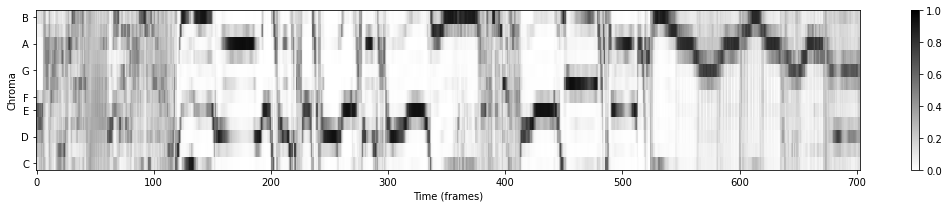
\includegraphics[width=\textwidth]{chromas/bo_cartero_trama_crudo.png}
        \caption{Navidad en las trincheras}
    \end{subfigure}
    \begin{subfigure}{\textwidth}
        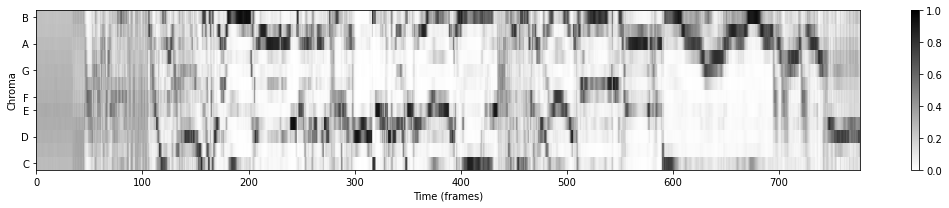
\includegraphics[width=\textwidth]{chromas/bo_cartero_trama_2_crudo.png}
        \caption{Cuarteto de nos}
    \end{subfigure}
    \caption{Cromas de la introducción de ``Bo cartero'' en cada disco}
    \label{fig:cromas_bo_cartero_ej}
\end{figure}

\subsection{DTW - Dynamic Time Warping}

El DTW es un algoritmo que permite cuantificar la similitud entre dos secuencias. Las secuencias no tienen por qué tener el mismo largo, por lo que dos realizaciones de la misma musica muestreadas a frecuencias diferentes, o tocadas a distinta velocidad, pueden ser reconocidas por este algoritmo. 

Utilizando una función de costo, se calcula una matriz de costo donde se compara cada trama de un cromagrama contra el resto del otro. Esta matriz actúa como un mapa de similitud entre las tramas del cromagrama, sobre el cual calcularemos el mejor camino de deformación (Warping Path). Este camino verifica ser el camino del extremo inferior izquierdo (principio de los cromagramas) al extremo superior derecho (fin de los cromagramas), monótono creciente (no retrocede temporalmente en ninguna de las tramas), que minimiza el costo acumulado. 

Se pueden agregar restricciones al camino para mejorar la sincronización, cambiando los posibles incrementos que puede tomar, o restringiendo ciertas partes del espacio. En la figura \ref{fig:distintos_DTW}, se observa el path obtenido con el DTW para los cromas de la figura \ref{fig:cromas_bo_cartero_ej}.

\begin{figure}[!htb]
    \centering
    \begin{subfigure}{0.49\textwidth}
        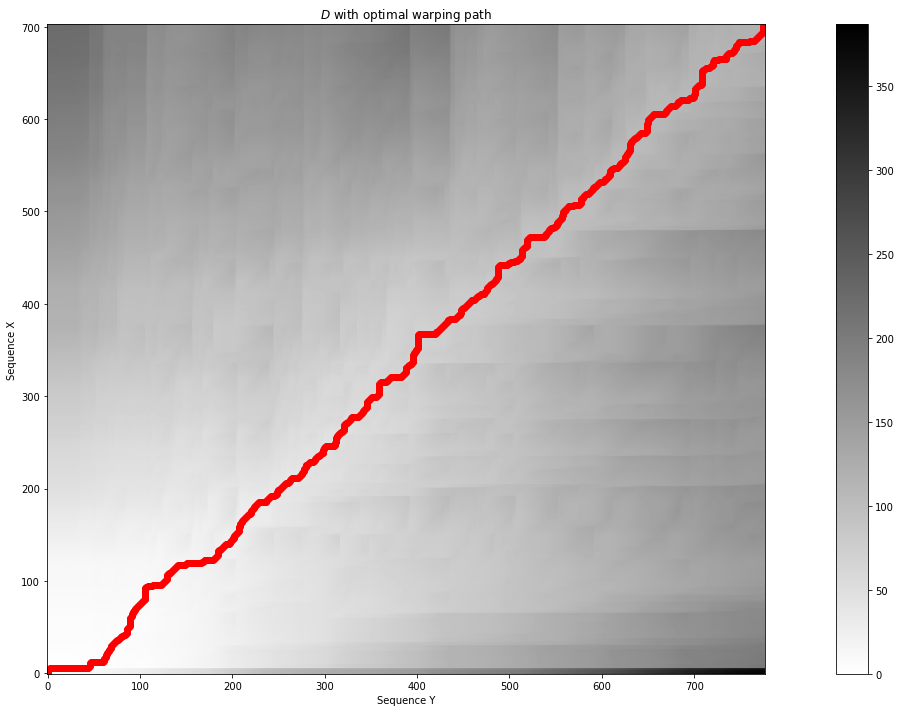
\includegraphics[width=\textwidth]{dtws/dtw_bo_cartero.png}
        \caption{DTW básico}
    \end{subfigure}
    \begin{subfigure}{0.49\textwidth}
        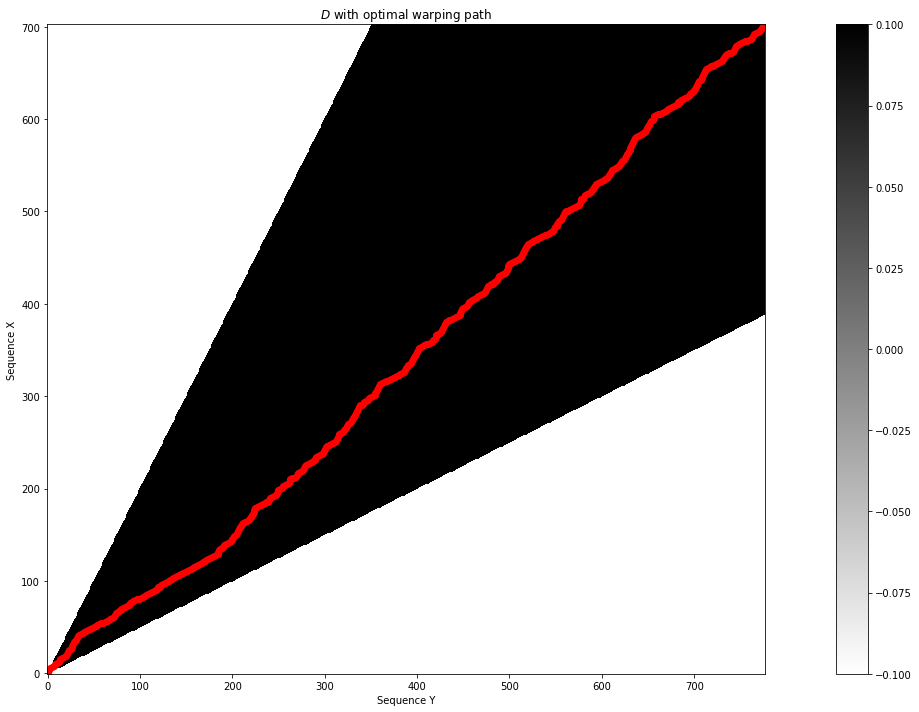
\includegraphics[width=\textwidth]{dtws/dtw_bo_cartero_step_size.png}
        \caption{DTW con step size $\{(1,2), (2,1), (1,1)\}$}
    \end{subfigure}
    \caption{Comparación de DTWs }
    \label{fig:distintos_DTW}
\end{figure}

Notar que cuando se varía el step size, es decir, cuanto puede aumentar varía la región que el path puede recorrer, por lo que se ahorra el cálculo de la matriz de confusión en estas regiones. El resultado en cuanto a distancia es $0.239$ para el DTW básico $0.280$ para el DTW con el step size cambiado. Hay un aumento del costo de sincronizar, pero se obtiene un camino menos sinuoso, lo cual es favorable a la hora de sincronizar. Estos compromisos deben ser evaluados según la aplicación. 

% CALCULO DE DISTANCIA

\section{Primera etapa}

\subsection{Búsqueda manual de covers}
En esta parte se aborda la detección de covers. 
En primer lugar se hace una inspección manual del corpus musical en búsqueda de versiones similares de una misma canción. Con eso se confecciona la lista presentada en la tabla \ref{canciones} en la que se identifican los covers en los dos discos que se tienen para el análisis. 

\begin{table}[!h]
\centering
\begin{tabular}{|l|l|}
\hline
\textbf{Otra Navidad en las Trincheras}  & \textbf{El Cuarteto de Nos}              \\
\hline
02. Solo un rumor       & 02. Solo un rumor       \\
05. El puton del barrio & 07. El puton del barrio \\
06. Eres una Chica muy Bonita   & 14. Eres una chica muy bonita \\
07. Bo cartero          & 04. Bo cartero          \\
08. Manfreddi       &   13. Manfreddi   \\
09. Nuevamente          & 06. Nuevamente    \\
11. Soy un Capón    & 15. Soy un capón  \\
12. Me agarre el pitito con el cierre & 18. Me agarre el pitito con el cierre (vivo) \\
\hline
\end{tabular}
\caption{Covers encontrados en los discos}
\label{canciones}
\end{table}

En los covers detectados hay gran variedad. En el caso de canciones como \textit{``Bo cartero''} y \textit{``Sólo un rumor''}, los cambios son principalmente en la calidad de la grabación (y de la banda) producto de casi 10 años de diferencia. En el caso de \textit{``El putón del barrio''} y \textit{``Me agarre el pitito con el cierre''} se tiene un cambio radical en al canción, donde en la primera se mantiene sólo la letra, y en la segunda se tiene una versión de estudio donde se usa un vocoder para dar la imagen de un niño cantando, contra una versión en vivo, donde se hace una versión acústica del tema (sin el vocoder y más lenta). El resto de los temas están en un intermedio, donde la mayoría de los cambios se dan por la mejora en calidad y una tendencia más instrumental en los temas.

Esto introduce una dificultad a la hora de implementar el clasificador de covers. La diferencia en la calidad de las mezclas, intensidad y calidad de la voz, intensidad de los instrumentos, presentan un desafío que hay que sortear. Esto es sin tener en cuenta los casos donde se reinventaron por completo los temas. A estas dificultades se le pueden sumar tres mas que quizás no son tan perceptibles al oído. 

\subsection{Tuning}

En primer lugar, el mapeo que se realiza a la hora de calcular el cromagrama parte de la premisa qué la música está afinada respecto a la escala de $A=440Hz$, pero puede no ser el caso. Pequeñas desafinaciones, que puede que no sean percibidas por el oyente, afectan el resultado del croma. La solución consiste en realizar un tuning para asegurarse de que se este en esa escala. El tuning se realiza dentro de la función de librosa que calcula el cromagrama, donde se realiza una estimación de la desafinación. Comienza con una búsqueda del pitch, utilizando un algoritmo de interpolación parabólica sobre la STFT, de donde obtiene una estimación de frecuencia fundamental en el tiempo. Con esta estimación se calcula la distancia a la frecuencia de la escala temperada más cercana para cada tiempo y se realiza un histograma. La distancia que tenga el mayor número de ocurrencias será la desviación respecto a la escala de $440Hz$.

Estudiemos la importancia de este afinamiento con la canción `` El puton del barrio" del álbum  ``Otra navidad en las trincheras" . En la figura \ref{tuning} se puede apreciar un cromagrama más difuminado cuando no se aplica afinamiento, por ejemplo entre los frames 200 y 250, donde la nota D aparece más nítida. Suponiendo que Roberto Musso está cantando un poquito fuera de tono, al no aplicarle el tuning, al chroma se le dificulta diferenciar entre la nota D y D\#. Este efecto se ve a lo largo de todo el cromagrama.

\begin{figure}[!h]
\centering
\begin{subfigure}{\textwidth}
    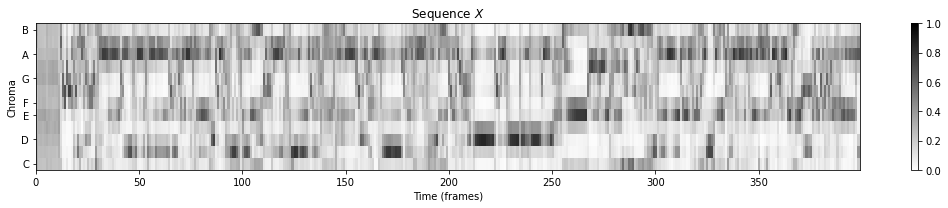
\includegraphics[width=\textwidth]{chromas/solo_un_rumor_sin.png}
    \caption{Sin tuning}
    \label{16_cropped}
\end{subfigure}
\vfill
\begin{subfigure}{\textwidth}
    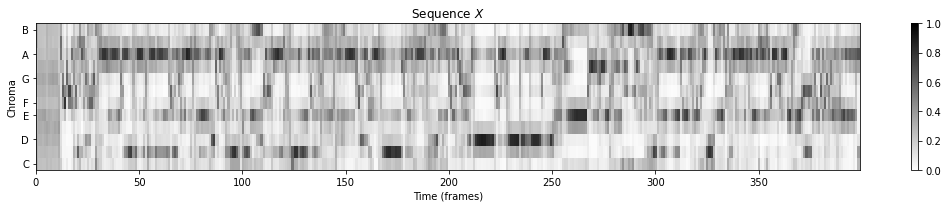
\includegraphics[width=\textwidth]{chromas/solo_un_rumor_tuning.png}
    \caption{Con tuning automático}
    \label{fig:16}
\end{subfigure}
\caption{Efecto de aplicar tuning en el cromagrama}
\label{tuning}
\end{figure}

\subsection{Cambio de tonalidad}

Otro problema es la posibilidad de tener canciones en diferentes tonalidades. Para ejemplificar este problema se tomo un fragmento de la canción ``Solo un rumor" y con el programa Audacity se detecto que se encontraba el tono en Fa, y utilizando herramientas de Audacity se la cambio a Do. Esta es una práctica muy común a la hora de hacer covers, donde muchas veces quién canta la nueva versión no tiene el mismo rango vocal que el autor original, o el nuevo estilo al que se la esta convirtiendo requiere esta translación en tono. 

Para resolver este problema existe una función compute\_optimal\_chroma\_shift de la biblioteca synctoolbox. La función prueba hacer el alineamiento con los 12 desplazamientos posibles del croma y devuelve la cantidad de shifts óptima que minimiza la distancia DTW. Luego se usa la función shift\_chroma\_vectors que realiza el corrimiento correspondiente. Para la canción que generamos de ejemplo, el shift óptimo es 6 (de Fa a Do). Los resultados se adjuntan en la figura \ref{corrimiento}.


\begin{figure}[!htb]
\centering
\begin{subfigure}{\textwidth}
    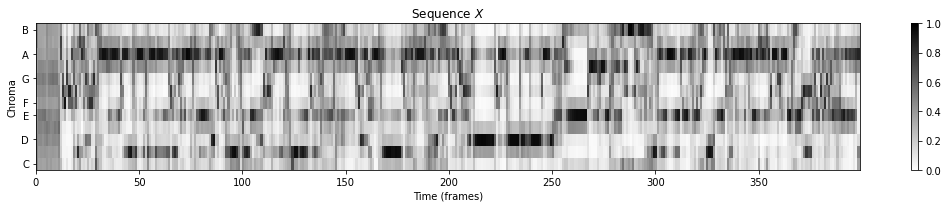
\includegraphics[width=\textwidth]{chromas/solo_un_rumor_ori.png}
    \caption{Cromagrama de Solo un rumor original}
    \label{fig:16}
\end{subfigure}
\vfill
\begin{subfigure}{\textwidth}
    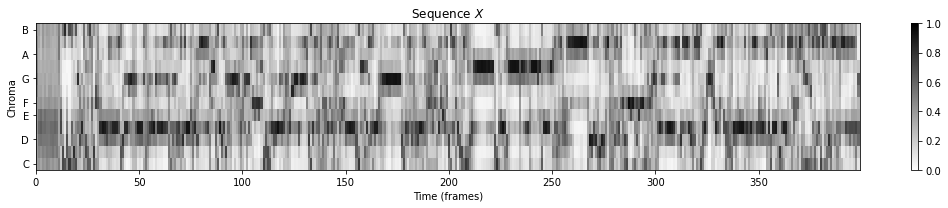
\includegraphics[width=\textwidth]{chromas/solo_un_rumor_do.png}
    \caption{Cromagrama de Solo un rumor en tono Do}
    \label{16_cropped}
\end{subfigure}
\vfill
\begin{subfigure}{\textwidth}
    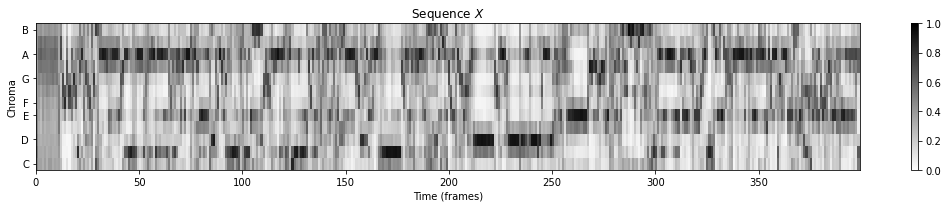
\includegraphics[width=\textwidth]{chromas/solo_un_rumor_do_shifted.png}
    \caption{Cromagrama de Solo un rumor en Do luego del optimal chroma shift}
    \label{16_cropped}
\end{subfigure}
\caption{Efecto de aplicar tuning en el cromagrama}
\label{corrimiento}
\end{figure}


\subsection{Normalización}

Por último tenemos las diferencias en la duración temporal de las excitaciones, causada por el uso de instrumentos distintos, o por la calidad de la grabación de dichos. La distribución de energía en el espectro también puede diferir por este motivo, por lo que, en función de cómo es el timbre, la representación del cromagrama va a variar. Aún así, sabemos que en la mayoría de los instrumentos (excepto percusivos) los armónicos están. Una forma de buscar estos armónicos que pueden quedar escondidos por instrumentos de mayor intensidad es aplicar compresión logarítmica.

A su vez no se tiene en cuenta la intensidad en función del tiempo. Distintos momentos de la canción pueden tener distintos volúmenes, por lo que si no se normaliza de alguna forma el cromagrama no va a ser una representación útil en todo instante de tiempo. En la figura \ref{normalizacion} se ve el resultado de aplicar distintas normalizaciones, viendo como a medida que se aumenta la norma se gana nitidez en cada trama. En la figura \ref{fig:16_sin_norma} se realizo una normalización tomando el máximo de todo el croma y dividiendo por ese valor para que pueda ser representado. Aún así muestra como no usar normalización trama a trama genera perdidas en algunas zonas de la canción, mientras la figura \ref{16_norma_2} se distinguen claramente todas las notas, pero las partes de silencio quedan bastante ruidosas.

\begin{figure}[!h]
\centering
\begin{subfigure}{\textwidth}
    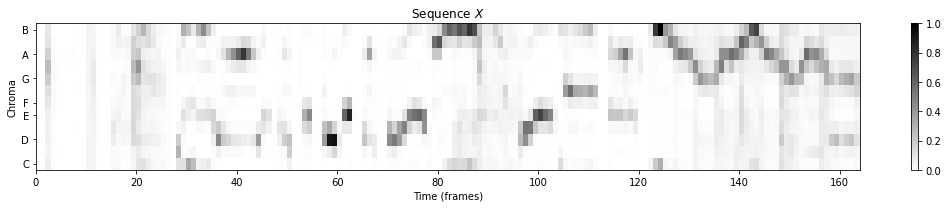
\includegraphics[width=\textwidth]{chromas/bo_cartero_sin.png}
    \caption{Cromagrama intro Bo cartero sin normalización}
    \label{fig:16_sin_norma}
\end{subfigure}
\vfill
\begin{subfigure}{\textwidth}
    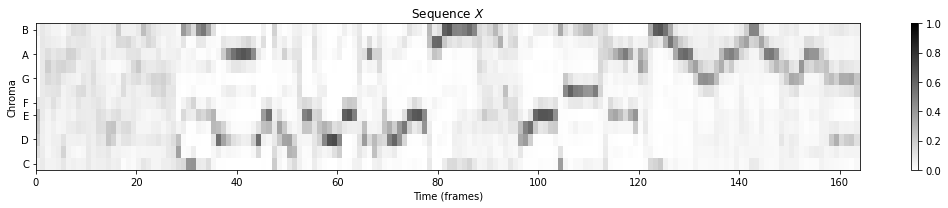
\includegraphics[width=\textwidth]{chromas/bo_cartero_con1.png}
    \caption{Cromagrama intro Bo cartero con normalización respecto a norma 1}
    \label{16_norma_1}
\end{subfigure}
\vfill
\begin{subfigure}{\textwidth}
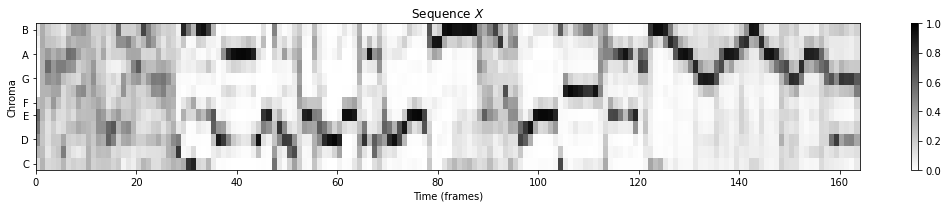
\includegraphics[width=\textwidth]{chromas/bo_cartero_con.png}
    \caption{Cromagrama intro Bo cartero con normalización respecto a norma 2}
    \label{16_norma_2}
\end{subfigure}
\caption{Efecto de aplicar normalización en el cromagrama}
\label{normalizacion}
\end{figure}

\subsection{Cromagrama final}

Además de tener en cuenta estos problemas, se realizó una limpieza general de los cromagramas siguiendo el tutorial de librosa \cite{Librosa}. Esta limpieza consiste en tres pasos
\begin{enumerate}
    \item primero se resaltan los componentes armónicos de la señal para separar mejor los sonidos armónicos de los percusivos
    \item se limpia el ruido haciendo un filtrado no local basado en vecinos mas cercanos
    \item se eliminan los transitorios y las discontinuidades horizontales con un filtro de mediana
\end{enumerate}

\begin{figure}[!h]
\centering
\begin{subfigure}{\textwidth}
    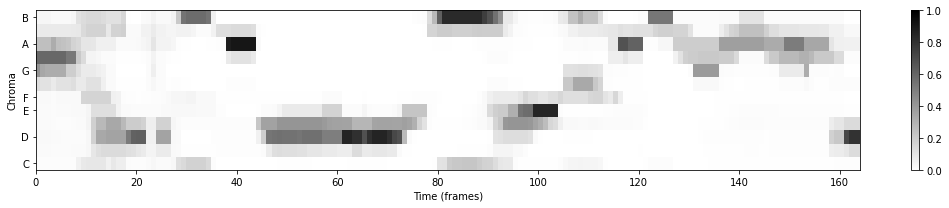
\includegraphics[width=\textwidth]{chromas/bo_cartero_1.png}
    \caption{``Otra navidad en las trincheras (1994)"}
    \label{bo_cartero1}
\end{subfigure}
\vfill
\begin{subfigure}{\textwidth}
    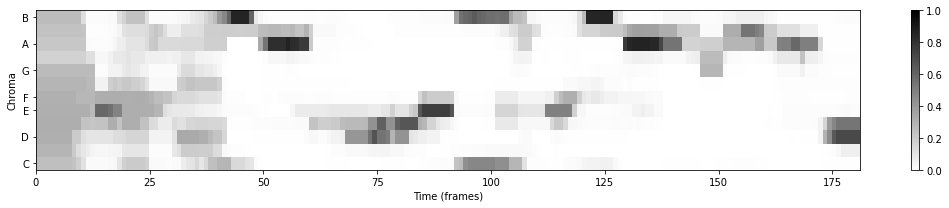
\includegraphics[width=\textwidth]{chromas/bo_cartero_2.png}
    \caption{``El cuarteto de Nos (2004)"}
    \label{bo_cartero2}
\end{subfigure}
\caption{Comparación cromagramas de la introducción de cada versión de``Bo cartero"}
\label{bo_cartero}
\end{figure}

\begin{figure}[!h]
\centering
\begin{subfigure}{\textwidth}
    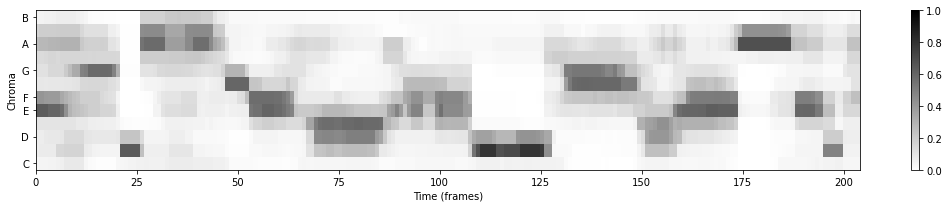
\includegraphics[width=\textwidth]{chromas/puton_barrio_1.png}
    \caption{``Otra navidad en las trincheras (1994)"}
    \label{puton_del_barrio1}
\end{subfigure}
\vfill
\begin{subfigure}{\textwidth}
    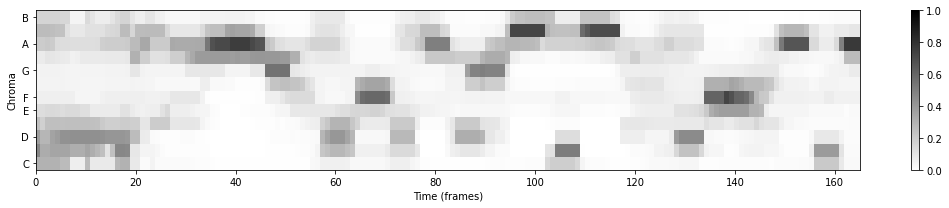
\includegraphics[width=\textwidth]{chromas/puton_barrio_2.png}
    \caption{``El cuarteto de Nos (2004)"}
    \label{puton_del_barrio2}
\end{subfigure}
\caption{Comparación cromagramas de la primer frase de cada versión de ``El puton del barrio"}
\label{puton_del_barrio}
\end{figure}

Es con todas estas consideraciones que se calcularon cromagramas que se utilizan como representación intermedia para aplicarles el algoritmo DTW. Se descarto el uso de compresión logarítmica, dado que no tuvo un impacto positivo en los cromas. Como una manera de familiarizarse con esta representación fue que se calcularon los cromagramas de fragmentos de los covers detectados en la tabla \ref{canciones}. Algunos ejemplos notables se adjuntan en las figuras \ref{bo_cartero} y \ref{puton_del_barrio}. En primer lugar, se observa que el cromagrama de bo cartero es mucho más simple que los reportados en figuras anteriores. Esta característica es deseable, porque mantiene solo la información más fundamental de la canción, atenuando por ejemplo vibratos o arreglos pequeños que podrían dificultar la detección.

Se ve como claramente los cromas de \ref{bo_cartero} presentan una similitud notable, pese a tener una diferencia en duración, mientras que en el caso de ``El putón del barrio'', figura \ref{puton_del_barrio}, los cromas no tienen mucha concordancia, coherente con lo que se mencionó al principio respecto al cambio radical que tiene esta canción de un albúm a otro.

\subsection{Distancia DTW}

Para comenzar a fijar los parámetros del DTW a usar, se entreno usando todos los covers mencionados en la tabla \ref{canciones} (quitando ``El putón del Barrio'' y ``Me agarre el pitito con el cierre'' por lo antes mencionado) junto con pares de canciones no covers al azar. Se busco que se tuviera mas o menos la misma cantidad de covers que canciones diferentes para maximizar la muestra minimizando el uso de recursos. Se experimento variando la función de costo, optando finalmente por la distancia coseno. También se varió los step size posibles, eligiendo $\{ (1,2), (2,1), (1,1) \}$ siempre que sea posible, y cuando no se halla solución se revierte a $\{(1,0), (0,1), (1,1)\}$. Se probo con restricciones globales, pero no se noto mejora, por lo que no se usaron.

Teniendo fijados los parámetros, se procedió a hacer la comparación todas las canciones de un disco contra todas las canciones del otro. Para optimizar, se calculo primero el croma grama de todas las canciones, y luego se generó una matriz con los resultados de la distancia DTW se muestran en la figura \ref{fig:distancias_allvall}. 

\begin{figure}[!htb]
    \centering
    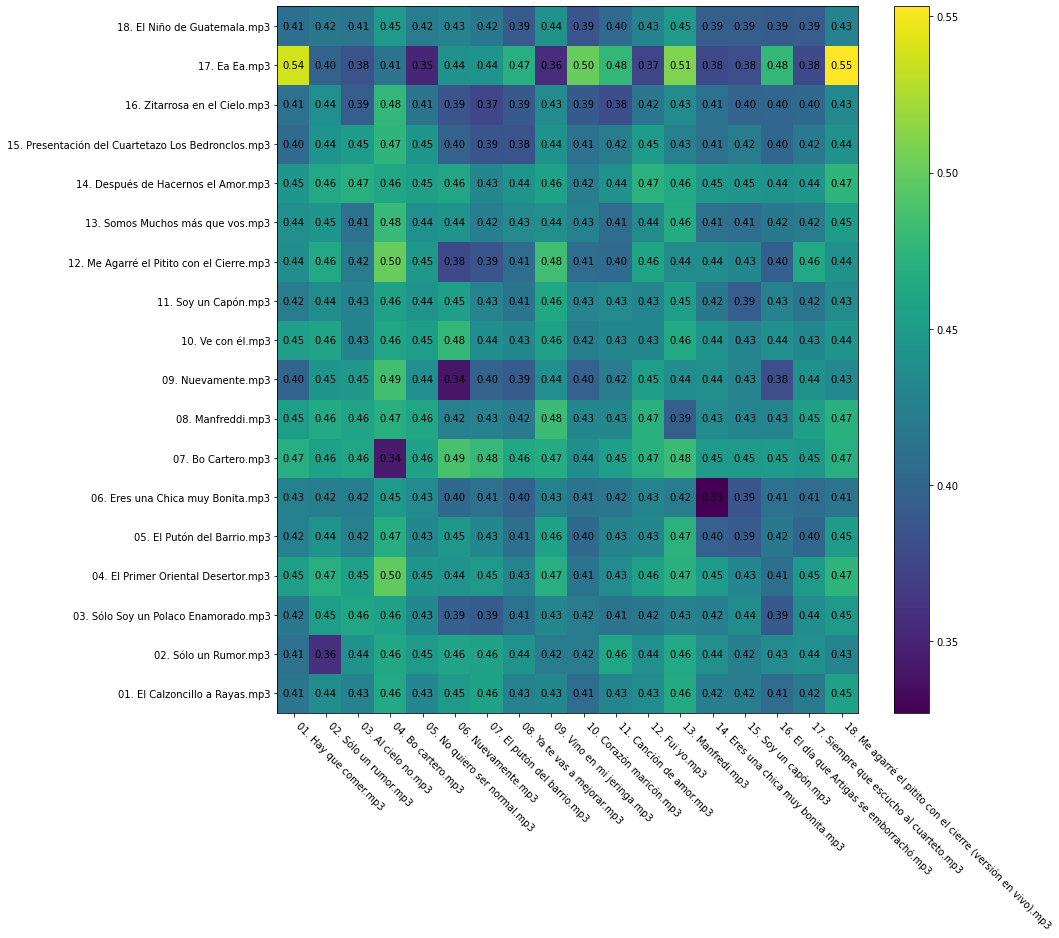
\includegraphics[width=\textwidth]{dtws/matrix_all_vs_all.png}
    \caption{Matriz con las distancias calculadas}
    \label{fig:distancias_allvall}
\end{figure}

Se observan ciertos imperfectos a la hora de calcular la distancias. ``Ea Ea'' presenta similitud con muchos temas, mientras que covers como ``Soy un capón'' o ``Manfreddi'' no obtienen valores mucho menores que otros otras comparaciones. Para resolver estos imperfectos requiere adentrarse más a fondo en técnicas tanto de representación por cromagramas como de alineación por DTW, pero para ser un primer acercamiento se obtuvo un resultado razonable.

La elección del umbral a partir del cual se considera una sospecha de cover va a depender de la aplicación. Si lo que se busca es un detector de plagio, por ejemplo, el umbral deberá ser alto para tener una baja tasa de falsos negativos. Si se quiere hacer recomendaciones en base a los gustos de una persona, el umbral deberá ser más restrictivo para qué no mezcle canciones que no tienen relación.


\section{Segunda etapa}

\subsection{Estudio de la canción elegida}

Para esta etapa se decidió utilizar las versiones de ``Bo carteros" que habían sido correctamente detectadas como cover en la etapa anterior con una distancia de $0.3433$. Escuchando las dos versiones, la primer diferencia notoria es en la velocidad de interpretación de las canciones siendo la versión del álbum ``El cuarteto de Nos" la más rápida. También hay diferencia en cuanto a la intensidad con la que se escuchan los instrumentos y la voz cantada principal, producto de la mejora de la calidad de grabación y la mezcla. A modo de ejemplo, en la sección instrumental alrededor de los 2 minutos de las canción, en la versión de ``Otra navidad en las trincheras" se escucha predominantemente una guitarra eléctrica junto a una acústica con la batería de fondo, mientras que en la otra versión se escucha la batería más alto y la solo hay una guitarra eléctrica.

Otra diferencia se escucha en la parte de la estrofa que comienza con ``Quizás se este haciendo dar", donde las voces tienen una cadencia muy distinta y además el acompañamiento es muy diferente. En la versión de ``Otra navidad en las trincheras" la batería se escucha muy poco y se escuchan acordes aislados de la guitarra mientras que en la otra versión se sigue igual que como se venía.  Por ultimo hay una diferencia de letra al final, en ``El cuarteto de Nos" la letra es ``si no vamos a hacerte terrible enema" mientras que en la otra versión es ``si no te vamos a hacer terrible enema". En cuanto a la terminación, la versión de ``Otra navidad en las trincheras" es mas abrupta que en el otro caso. 

\subsection{Alineación}

%Es con estas tramas que se se muestran las alineaciones en el tiempo y de espectrograma.

Para realizar el alineamiento entre las secuencias se decidió probar en primera instancia con la trama de la introducción ya usadas a lo largo de este informe. El alineamiento se realiza con la función hps\_tsm de libtsm. Esta función realiza una separación entre componentes armónicos y percusivos, luego realiza un phase vocoder para los componentes armónicos y un WSOLA para los percusivos, para modificar la duración temporal sin alterar destructivamente el espectro (o lo menos posible). Ambas modificaciones temporales las hace siguiendo una función alpha, que en este caso es el camino obtenido con el DTW. 

Para realizar la separación se usa la función hps de libtsm que aplica, sobre el espectrograma, un filtro de mediana en el sentido vertical para quedarse con las componentes percusivas, y un filtro de mediana horizontal para quedarse con los armónicos. 

El phase vocoder es una técnica que permite hacer modificaciones en la escala temporal sin tener modificaciones de pitch. La idea es poder modelar la señal con armónicos (es decir de manera sinusoidal), es por eso que solo sirve para este tipo de componentes. El algoritmo del phase vocoder realiza una interpolación de orden 1 del path y luego la evalúa en las posiciones de la ventana de síntesis. Con eso saca las posiciones de las ventanas de análisis de la entrada. Luego va frame a frame en la STFT y hace el desdoblamiento de fase para luego calcular la inversa de la STFT con la fase corregida. 
Por otro lado, de acuerdo a \cite{WSOLA}, en el algoritmo WSOLA la idea es la misma que con OLA pero dando un margen de movimiento a cada ventana antes de superponerlas de manera que la superposición quede lo mas parecida posible (en el sentido de la correlación cruzada). 

Al momento de implementar la alineación, se utilizó como referencia los resultados obtenidos con el notebook \textit{sync\_audio\_audio\_full.ipynb} del repositorio de GitHub \cite{GitHub} de la biblioteca SyncToolbox. Hay dos diferencias fundamentales con ese procedimiento, la primera es el computo de DLNCO features y luego la aplicación de un algoritmo llamado MrMsDTW para obtener el warping path. El alineamiento es igual. Las DLNCO features están basadas en las características del chroma, pero que buscan aumentar la robustez de las mismas. De acuerdo a Ewert, S\cite{DLNCO}, la idea es usar el chroma onset para tener en cuenta la intensidad de los sonidos, y luego aplicar un filtrado normalizador adaptivo local con decaimiento, lo que genera unas features con mayor información. La gracia es que a la hora de hacer el DTW, estas nuevas features ajustan localmente el path y dan mas precisión temporal. 
El algoritmo MrMsDTW es un DTW con memoria restringida y multi escala. Según Thomas Pratzlich \cite{MrMs}, se busca disminuir el costo de memoria del DTW original utilizando una solución multi-escala en la cual primero se calcula el path en una grilla de resolución gruesa, luego se proyecta a una grilla con mayor resolución y ahí se refina usando  una restricción tubular. La parte de restringir la memoria se basa en poner una cota superior a la cantidad de celdas que se pueden usar para el computo del algoritmo. 

Para la utilización de nuestro path se tuvieron que hacer algunas modificaciones tomando en cuenta de que los cromagramas construidos habían sido refinados para tener un buen desempeño en el problema de detección de covers. Se construyeron teniendo la distancia en mente y no las implicancias temporales de las decisiones tomadas. 

En cuanto al cálculo del cromagrama el único cambio que se consideró pertinente fue el cambio de resolución de la STFT y, tomando como referencia el notebook mencionado anteriormente, se eligió un hop size de 512 y NFFT de 1024. Se quito además la limpieza presentada utilizada en la parte anterior, donde se habían representado solo los componentes armónicos y se habían realizado dos tipo de filtrado. Esta información que se descarto en la detección de covers puede ser muy útil para el alineamiento, dejando las marcas temporales que dan los elementos percusivos, Por último, se aseguró que el path obtenido fuese estrictamente creciente para evitar problemas de repetición, lo cuál ya se estaba haciendo en la detección de covers. 

Con estas consideraciones se logró un resultado satisfactorio comparando con lo obtenido con MrMsDTW. En la figura \ref{correspondencia} se adjunta la correspondencia temporal entre las introducciones de ``Bo cartero" para el path calculado con DTW y las consideraciones pertinentes. En este caso el path es mucho mas suave que en la parte anterior y la distancia es 0.23. 

\begin{figure}[!h]
    \centering
    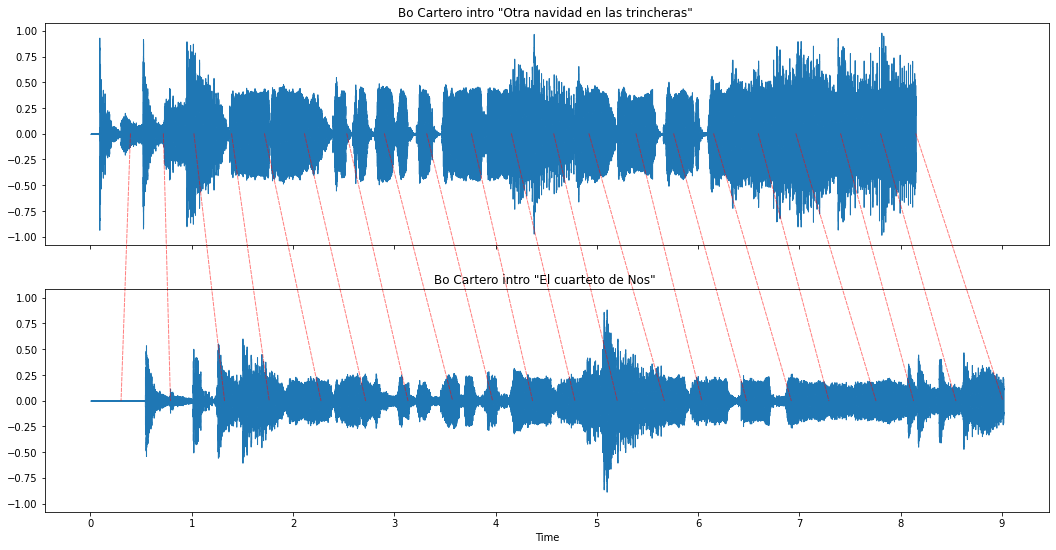
\includegraphics[width=\textwidth]{Alineamientos/alineamiento.png}
    \caption{Correspondencia temporal entre tramas de la introducción de Bo Cartero}
    \label{correspondencia}
\end{figure}

En la figura \ref{espectrogramas} se muestran los espectrogramas de las versiones alineadas, y se puede acceder a las canciones alineadas en este \href{https://drive.google.com/drive/folders/1IeRXLXKivI5VXjGnCVVK31Mhy6xFf_kc?usp=sharing}{link}. En estos se pueden ver varias similitudes y algunas diferencias, en especial al comienzo donde ya preceptivamente se puede notar una gran distorsión, hasta que comienzan las voces y tenemos una sincronización más clara. A su vez la batería parece estar bastante sincronizada, cosa que se ve en la figura \ref{espectrogramas} en la banda entorno a los 4s. Esto es una mejora respecto a los resultados obtenidos con el algoritmo MrMsDTW, en el cual se logra sincronizar bien la voz pero no la batería. 

\begin{figure}[!htb]
    \centering
    \begin{subfigure}{0.49\textwidth}
        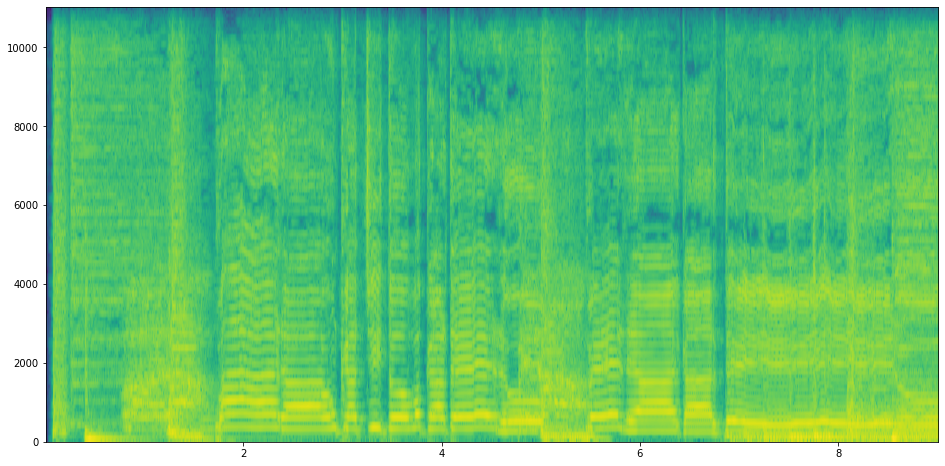
\includegraphics[width=\textwidth]{Alineamientos/espectro_y.png}
        \caption{Trama alineada}
    \end{subfigure}
    \begin{subfigure}{0.49\textwidth}
        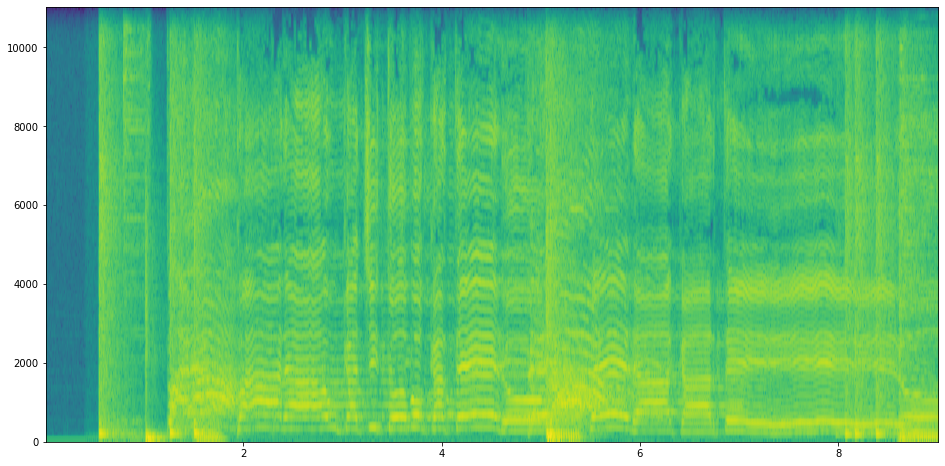
\includegraphics[width=\textwidth]{Alineamientos/espectro_audio.png}
        \caption{Trama de referencia}
    \end{subfigure}
    \caption{Comparación de espectrogramas alineados.}
    \label{espectrogramas}
\end{figure}

Los resultados de la sincronización completa con el path obtenido con DTW auditivamente son relativamente buenos, estos se pueden escuchar en este \href{https://drive.google.com/drive/folders/1IeRXLXKivI5VXjGnCVVK31Mhy6xFf_kc?usp=sharing}{link}. En primer lugar hay una buena superposición de la voz, aunque la batería se desfasa por momentos. A su vez cabe destacar que las mayores diferencias se escuchan en los lugares donde se habían notado las mayores diferencias que se detallaron anteriormente, sobre todo en la parte instrumental y los versos después de eso.
Sobre los comentarios acerca del final de las canciones, cabe destacar como claramente se escucha muy bien en las palabras que coinciden (``terrible enema'') y muy mal en las diferentes (``vamos a hacerte'' vs ``te vamos a hacer''). 

Además, de poder decir perceptivamente si se escucha bien o no, es importante establecer una medida de desempeño mas objetiva. Para eso se calcula el beat, dado que al alinear secuencias temporales, el beat debería ser algo que coincide. Se calculan los tiempos donde se dan los beats usando el beat\_tracker de Librosa. Este algoritmo usa programación dinámica para resolver el problema en tres instancias. Primero se calcula la intensidad con la cual empieza cada nota, después se estima el tempo con la correlación entre las estimaciones de los comienzos, y por ultimo se eligen los picos de la intensidad que sean consistentes con el tempo estimado. 
La idea para establecer una métrica de desempeño es primero tener una estimación de donde se dan los beats para la señal editada respecto a donde están en la señal original con la que se alineo. Por eso se realiza la resta y se presenta un histograma con las distancias obtenidas para cada beat, que se presenta en la figura \ref{histograma}. Se puede ver, por ejemplo, donde se da el máximo de ocurrencias y tomar ese como la desviación del beat. Por último resta definir algún umbral para poder establecer cual es el límite en la desviación que permite considerar un buen o mal alineamiento. 

\begin{figure}[!h]
    \centering
    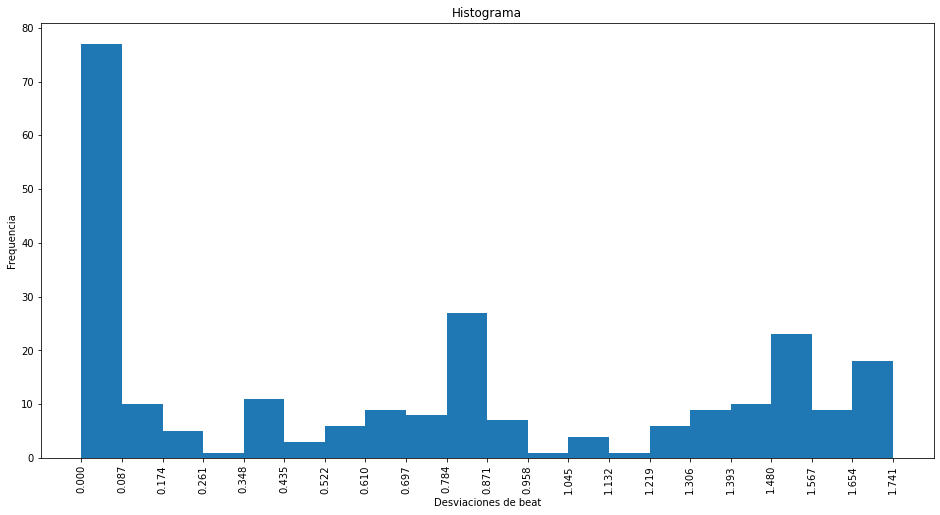
\includegraphics[width=0.80\textwidth]{histograma.png}
    \caption{Histograma de distancias entre beats}
    \label{histograma}
\end{figure}

En este caso, se puede considerar que la mayor cantidad de ocurrencias se da entre 0 y 0.087s. Si se establece un umbral de 100ms, se puede considerar un buen alineamiento. Sin embargo, para una mejor evaluación se podrían tener en cuenta los otros picos del histograma, por ejemplo en este caso, hay algunos picos a mas de 1s, eso es reflejo de la mala sincronización que se escucha por momentos. 

\section{Conclusión}
En cuanto a la primera etapa, se logró implementar un detector de covers con un desempeño satisfactorio. Se pudo evaluar la influencia de los parámetros al tratar de separar los covers del resto de comparaciones. También se logró bajar el costo computacional para poder realizar todas las comparaciones contra todas en tiempo razonable. 

En cuanto a la segunda parte, se pudo que parámetros impactan en el alineamiento y la diferencia con las consideraciones que se habían hecho para el calculo de distancias. A su vez, se pudo generar un alineamiento con el path calculado a partir de las features y DTW originales que se pudo comparar con el calculado a través de MrMsDTW. Por último también se llego a una manera de evaluar el alineamiento de manera objetiva que da lugar a muchas mejoras.   

Los desafíos planteados sirvieron para ver cómo herramientas de procesamiento de audio y de estimación temporal pueden ser utilizadas para abordar problemas distintos, que pese a que a priori parecen estar muy relacionados, las implementaciones se diferencian en aspectos claros de diseño. Ambos resultados tienen lugar para ser mejorados, siguiendo experimentando con los parámetros disponibles y explorando técnicas más complejas, como el cromagrama multiresolución.

\newpage
\section{Link a notebooks y audios}
El link es : \url{https://drive.google.com/drive/folders/1IeRXLXKivI5VXjGnCVVK31Mhy6xFf_kc?usp=sharing}

\bibliographystyle{plain}
\bibliography{refs}

\end{document}